\documentclass[12pt]{article}
\usepackage{ctex}
\usepackage{amsmath,amsthm}
\usepackage{graphicx,float}
\usepackage{fancyhdr}
\usepackage{array}
\usepackage[a4paper, total={7in,9in}]{geometry}

\graphicspath{{../image/}}

\renewcommand{\arraystretch}{1.8}

\fancyhf{}
\fancyhf[HL]{升中四暑期課程}
\fancyhf[FR]{P.\thepage}

\newtheorem*{theorem}{定理}
\newtheorem{example}{示例}

\begin{document}
    \pagestyle{fancy}
    \begin{center}
        \textbf{因數分解}
    \end{center}

    回顧因數分解概念,根據我們在小學學到的知識,某個數字(如18)的因數可用下列方式表示: \begin{align*}
        18&=1\times 18\\
        &=2\times 9\\
        &=3\times 6
    \end{align*}
    因此,在這個例子中,我們有 $1,2,3,6,9,18$ 作為 $18$ 的因子。同樣地,當我們進入多項式的討論時,因數分解的概念仍然有效,但因式分解的運算會變得不清楚,而需要對多項式本質有更多理解。

    觀察下列算式,已知 \begin{align*}
        x\cdot x=x^2
    \end{align*} 因此\begin{align*}
        x^2-2x&=x(x-2)\\
        x^3+4x^2&=x^2(x+4)
    \end{align*}

    若認為上面的表達式有點含糊,回憶分配律:\begin{align*}
        a(b+c)&=ab+ac\\
        (a+b)c&=ac+ab
    \end{align*} 並將倒推表達式。注意:因式分解只是展開數式的反向操作。\begin{align*}
        x(x-2)&=x\cdot x-x\cdot 2\\
        &=x^2-2x\\
        x^2(x+4)&=x^2\cdot x+x^2\cdot 4\\
        &=x^3+4x^2
    \end{align*}

    由於 $x^2\cdot x$ 可被視爲 $x\cdot x\cdot x$, 因此 3 個 $x$ 相乘可得 $x^3$.

    然而,並非每個多項式都像我們所看到的那樣簡單。對於物理學中存在的一些表達式,我們會遇到類似這樣的情況:\begin{align*}
        x^2+3x+4&=0
    \end{align*}

    我們有不同的方法以求$x$的值。接下來將使用之前學過的恆等式。

    讓我們先溫習一下我們對因式分解的理解。
    \subsection*{習題}
    \begin{enumerate}
        \item 例出下列數字的所有因子,包括負數:\begin{align*}
            &a)\ 4&&b)\ 6&&c)\ 12&&d)\ 15\\
            &e)\ 32&&f)\ 44&&g)\ 52&&h)\ 80
        \end{align*}
        \item 對下列各項進行質因數分解:\begin{align*}
            &a)\ 4&&b)\ 6&&c)\ 12&&d)\ 15\\
            &e)\ 32&&f)\ 44&&g)\ 52&&h)\ 80
        \end{align*}
        \item 因式分解:\begin{align*}
            &a)\ x^2+x&&b)\ x-xy&&c)\ x^4+2x^2+2x&&d)\ x^3-2x
        \end{align*}
    \end{enumerate}

    \begin{center}
        \textbf{以恆等式進行因式分解}
    \end{center}

    回顧以下展開式:\begin{align*}
        (x+y)^2&=x^2+2xy+y^2\\
        (x-y)^2&=x^2-2xy+y^2\\
        (x+y)(x-y)&=x^2-y^2
    \end{align*}

    我們應該注意到,等號是雙向有意義的,也就是說,每當左手邊等於右手邊,右手邊就立即等於左手邊。因此,我們可能會從相反的方向來看上面的情況。\begin{align*}
        x^2+2xy+y^2&=(x+y)^2\\
        x^2-2xy+y^2&=(x-y)^2\\
        x^2-y^2&=(x+y)(x-y)
    \end{align*}

    這稱為\textbf{恆等式因式分解}。

    \begin{example}
        因式分解 $x^2+2x+1$.
    \end{example}
    \textit{ 解. }\begin{align*}
        x^2+2x+1&=(x)^2+2(x)(1)+(1)^2\\
        &=(x+1)^2
    \end{align*}

    \begin{example}
        因式分解 $x^2+4x+4$.
    \end{example}
    \textit{ 解. }\begin{align*}
        x^2+4x+4&=(x)^2+2(x)(2)+(2)^2\\
        &=(x+2)^2
    \end{align*}

    \begin{example}
        因式分解 $x^2-2x+1$.
    \end{example}
    \textit{ 解. }\begin{align*}
        x^2-2x+1&=(x)^2-2(x)(1)+(1)^2\\
        &=(x-1)^2
    \end{align*}

    \begin{example}
        因式分解 $x^2-4x+4$.
    \end{example}
    \textit{ 解. }\begin{align*}
        x^2-4x+4&=(x)^2-2(x)(2)+(2)^2\\
        &=(x-2)^2
    \end{align*}

    \begin{example}
        因式分解 $x^2-1$.
    \end{example}
    \textit{ 解. }\begin{align*}
        x^2-1&=(x)^2-(1)^2\\
        &=(x+1)(x-1)
    \end{align*}

    \begin{example}
        因式分解 $x^2-9$.
    \end{example}
    \textit{ 解. }\begin{align*}
        x^2-9&=(x)^2-(3)^2\\
        &=(x+3)(x-3)
    \end{align*}

    讓我們運用恆等式做些簡單的因式分解練習。

    \subsection*{習題}
    \begin{enumerate}
        \item 因式分解:\begin{align*}
            &a)\ x^2+6x+9&&b)\ x^2+8x+16&&c)\ x^2+10x+25&&d)\ x^2+16x+64\\
            &e)\ 2x^2+12x+18&&f)\ 4x^2+32x+64&&g)\ 6x^2+60x+150&&h)\ 8x^2+128x+512\\
            &i)\ x^3+6x^2+9x&&j)\ x^5+8x^4+16x^3&&k)\ x^8+10x^6+25x^4&&l)\ x^9+16x^5+64x\\
        \end{align*}
        \item 因式分解:\begin{align*}
            &a)\ x^2-6x+9&&b)\ x^2-8x+16&&c)\ x^2-10x+25&&d)\ x^2-16x+64\\
            &e)\ 2x^2-12x+18&&f)\ 4x^2-32x+64&&g)\ 6x^2-60x+150&&h)\ 8x^2-128x+512\\
            &i)\ x^3-6x^2+9x&&j)\ x^5-8x^4+16x^3&&k)\ x^8-10x^6+25x^4&&l)\ x^9-16x^5+64x\\
        \end{align*}
        \item 因式分解:\begin{align*}
            &a)\ x^2-9&&b)\ x^2-16&&c)\ x^2-25&&d)\ x^2-64\\
            &e)\ 2x^2-18&&f)\ 4x^2-64&&g)\ 6x^2-150&&h)\ 8x^2-512\\
            &i)\ x^3-9x&&j)\ x^5-16x^3&&k)\ x^8-25x^4&&l)\ x^9-64x\\
        \end{align*}
        \item 因式分解:\begin{align*}
            &a)\ x^2+2ax+a^2&&b)\ x^2+8x+16-b^2\\
            &c)\ x^2+10x+25-y^2+2yc-c^2&&d)\ ax^2+16a^2x+64a^3\\
            &e)\ 2x^2+12xy+18y^2&&f)\ 4(x+y)^2+32(x^2-y^2)+64(x-y)^2
        \end{align*}
    \end{enumerate}

    \begin{center}
        \textbf{以更多恆等式進行因式分解}
    \end{center}

    為提高對因式分解的認知,我們將學習更多恆等式式以更熟練地運用它們。

    我們已有二次多項式,所以我們可以進階到三次多項式\begin{align*}
        (x+y)^3&=x^3+3x^2y+3xy^2+y^3\\
        (x-y)^3&=x^3-3x^2y+3xy^2-y^3\\
        (x+y)(x^2-xy+y^2)&=x^3+y^3\\
        (x-y)(x^2+xy+y^2)&=x^3-y^3
    \end{align*}

    為清晰起見,我們將為其提供一個證明。\begin{enumerate}
        \item 對於 $(x+y)^3=x^3+3x^2y+3xy^2+y^3$:\begin{align*}
            (x+y)^3&=(x+y)(x+y)^2\\
            &=(x+y)(x^2+2xy+y^2)\\
            &=x^3+3x^2y+3xy^2+y^3
        \end{align*}
        \item 對於 $(x-y)^3=x^3-3x^2y+3xy^2-y^3$:\begin{align*}
            (x-y)^3&=(x-y)(x-y)^2\\
            &=(x-y)(x^2-2xy+y^2)\\
            &=x^3-3x^2y+3xy^2-y^3
        \end{align*}
        \item 對於 $(x+y)(x^2-xy+y^2)=x^3+y^3$:\begin{align*}
            (x+y)(x^2-xy+y^2)&=x^3+x^2y-x^2y-xy^2+xy^2+y^3\\
            &=x^3+y^3
        \end{align*}
        \item 對於 $(x-y)(x^2+xy+y^2)=x^3-y^3$:\begin{align*}
            (x-y)(x^2+xy+y^2)&=x^3-x^2y+x^2y-xy^2+xy^2-y^3\\
            &=x^3-y^3
        \end{align*}
    \end{enumerate}
    
    讓我們通過一些例子來提升我們對其原理的熟練度。

    \begin{example}
        因式分解 $x^3+3x^2+3x+1$.
    \end{example}
    \textit{ 解. }\begin{align*}
        x^3+3x^2+3x+1&=(x)^3+3(x)^2(1)+3(x)(1)^2+(1)^3\\
        &=(x+1)^3
    \end{align*}

    \begin{example}
        因式分解 $x^3+6x^2+12x+8$.
    \end{example}
    \textit{ 解. }\begin{align*}
        x^3+6x^2+12x+8&=(x)^3+3(x)^2(2)+3(x)(2)^2+(2)^3\\
        &=(x+2)^3
    \end{align*}

    \begin{example}
        因式分解 $x^3-3x^2+3x-1$.
    \end{example}
    \textit{ 解. }\begin{align*}
        x^3-3x^2+3x-1&=(x)^3-3(x)^2(1)+3(x)(1)^2-(1)^3\\
        &=(x-1)^3
    \end{align*}

    \begin{example}
        因式分解 $x^3-6x^2+12x-8$.
    \end{example}
    \textit{ 解. }\begin{align*}
        x^3-6x^2+12x-8&=(x)^3-3(x)^2(2)+3(x)(2)^2-(2)^3\\
        &=(x-2)^3
    \end{align*}

    \begin{example}
        因式分解 $x^3+1$.
    \end{example}
    \textit{ 解. }\begin{align*}
        x^3+1&=(x)^3+(1)^3\\
        &=(x+1)(x^2-x+1)
    \end{align*}

    \begin{example}
        因式分解 $x^3+8$.
    \end{example}
    \textit{ 解. }\begin{align*}
        x^3+8&=(x)^3+(2)^3\\
        &=(x+2)(x^2-2x+4)
    \end{align*}

    \begin{example}
        因式分解 $x^3-1$.
    \end{example}
    \textit{ 解. }\begin{align*}
        x^3-1&=(x)^3-(1)^3\\
        &=(x-1)(x^2+x+1)
    \end{align*}

    \begin{example}
        因式分解 $x^3-8$.
    \end{example}
    \textit{ 解. }\begin{align*}
        x^3-8&=(x)^3-(2)^3\\
        &=(x-2)(x^2+2x+4)
    \end{align*}

    現在我們對3次多項式因式分解有了認識,讓我們做些基本的恆等式練習。

    \subsection*{習題}
    \begin{enumerate}
        \item 因式分解:\begin{align*}
            &a)\ x^3+9x^2+27x+27&&b)\ x^3+12x^2+48x+64&&c)\ x^3+15x^2+75x+125\\
            &d)\ 2x^3+18x^2+54x+54&&e)\ 3x^3+36x^2+144x+192&&f)\ 5x^3+75x^2+375x+625\\
        \end{align*}
        \item 因式分解:\begin{align*}
            &a)\ x^3-9x^2+27x-27&&b)\ x^3-12x^2+48x-64&&c)\ x^3-15x^2+75x-125\\
            &d)\ 2x^3-18x^2+54x-54&&e)\ 3x^3-36x^2+144x-192&&f)\ 5x^3-75x^2+375x-625\\
        \end{align*}
        \item 因式分解:\begin{align*}
            &a)\ x^3+27&&b)\ x^3+64&&c)\ x^3+125\\
            &d)\ 2x^3+54&&e)\ 3x^3+192&&f)\ 5x^3+625\\
        \end{align*}
        \item 因式分解:\begin{align*}
            &a)\ x^3-27&&b)\ x^3-64&&c)\ x^3-125\\
            &d)\ 2x^3-54&&e)\ 3x^3-192&&f)\ 5x^3-625\\
        \end{align*}
    \end{enumerate}

    \begin{center}
        \textbf{以十字相乘法進行因式分解}
    \end{center}

    從現在開始,我們將深入探究一個重要問題:如何解以下形式: $$x^2+px+q$$ 或為更廣汎的形式 $$ax^2+bx+c$$ 的二次方程? 假設 $x^2+px+q$ 可被分解爲 $$(x+a)(x+b)$$ 就相當於說 $$(x+a)(x+b)=x^2+px+q$$ 也就是説 $$x+(a+b)x+ab=x^2+px+q$$

    比較同類項,可見 \begin{align*}
        \begin{cases}
            a+b=p\\
            ab=q
        \end{cases}
    \end{align*}

    這給了我們一個提示,我們應先分解常數 $q$ 再利用$a+b=p$求得 $a,b$ 的正確值。

    總結步驟:\begin{enumerate}
        \item 通過比較同類項,求 $p,q$ 的值。
        \item 嘗試寫出q的每對因子。
        \item 檢查每對因子的和。 如符合 $a+b=p$,則為正確答案。
        \item 寫下 $(x+a)(x+b)$。
    \end{enumerate}

    \begin{example}
        因式分解 $x^2+4x+3$.
    \end{example}

    \textit{ 解.}1:求 $p$ 和$q$.
    \begin{align*}
        p=4, q=3
    \end{align*}
    \indent \indent 2:分解 $q$ (包含負數因子對).
    \begin{align*}
        3&=1\cdot 3\\
        &=(-1)\cdot(-3)
    \end{align*}
    \indent \indent 3:檢查 $a+b=p$ (包括負數因子對).
    \begin{align*}
        1+3&=4\\
        (-1)+(-3)&=-4
    \end{align*}
    \indent \indent \indent 由於 $p=4$,所以 $a=1,b=3$為正確答案\\
    \indent \indent 4:總結。
    \begin{align*}
        x^2+4x+3=(x+1)(x+3)
    \end{align*}

    我們應確保因式分解後的表達式可以展開為原本的多項式。\begin{align*}
        (x+1)(x+3)&=x(x+3)+(x+3)\\
        &=x^2+3x+x+3\\
        &=x^2+4x+3
    \end{align*}

    這說明我們的步驟正確。有數學家認為上述步驟可以有更緊凑的表示方式。這個方法我們將其稱為\textbf{十字相乘法}。
    
    \begin{example}
        利用十字相乘法因式分解 $x^2+4x+3$。
    \end{example}

    \textit{ 解.}由於 $3=1\cdot 3=(-1)\cdot(-3)$,
    \begin{figure}[H]
        \centering
        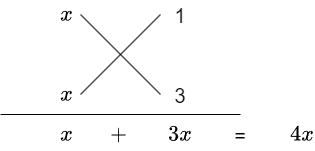
\includegraphics[scale=0.6]{cross-method}
    \end{figure}
    \indent \indent 即 $x^2+4x+3=(x+1)(x+3)$。

    我們可以通過以下練習來熟習十字相乘法的運用。

    \subsection*{習題}
    \begin{enumerate}
        \item 以十字相乘法因式分解:\begin{align*}
            &a)\ x^2+6x+8&&b)\ x^2+9x+18&&c)\ x^2+7x+6\\
            &d)\ x^2-6x+8&&e)\ x^2-9x+18&&f)\ x^2-7x+6\\
            &g)\ x^2+6x-27&&h)\ x^2+9x-22&&i)\ x^2+7x-30\\
            &j)\ x^2-6x-27&&k)\ x^2-9x-22&&l)\ x^2-7x-30
        \end{align*}
        \item 以十字相乘法因式分解:\begin{align*}
            &a)\ 2x^2+12x+16&&b)\ 3x^2+27x+54&&c)\ 5x^2+35x+30\\
            &d)\ 7x^2-42x+56&&e)\ -11x^2+99x-198&&f)\ -3x^2+21x-18
        \end{align*}
    \end{enumerate}

    \begin{center}
        \textbf{以因式分解法解二次方程}
    \end{center}

    為解二次方程,我們得知以下幾點\begin{theorem}
        若 $ab=0$, 則 $a=0$ 或 $b=0$。
    \end{theorem}

    從以上可見,若 $(x-\alpha)(x-\beta)=0$,則 $x-\alpha=0$ 或 $x-\beta=0$。因此方程的 \textbf{解} 為 $x=\alpha$ 或 $x=\beta$.

    \begin{example}
        解 $x^2-4x+3=0$.
    \end{example}

    \textit{ 解. }通過因式分解,可得 $(x-1)(x-3)=0$,因此 $x=1$ 或 $x=3$ 為方程的解。

    \begin{example}
        解 $x^2+4x+3=0$.
    \end{example}

    \textit{ 解. }通過因式分解,可得 $(x+1)(x+3)=0$,因此 $x=-1$ 或 $x=-3$ 為方程的解。

    當我遇到方程有兩個根,而兩個根是重複的話,我們只需列明其中一個根即可。

    \begin{example}
        解 $x^2+4x+4=0$.
    \end{example}

    \textit{ 解. }通過因式分解,可得 $(x+2)^2=0$,則 $x=-2$ 是唯一解

    \subsection*{習題}
    \begin{enumerate}
        \item 解方程:\begin{align*}
            &a)\ 2x^2+12x+16=0&&b)\ 3x^2+27x+54=0&&c)\ 5x^2+35x+30=0\\
            &d)\ 7x^2-42x+56=0&&e)\ -11x^2+99x-198=0&&f)\ -3x^2+21x-18=0
        \end{align*}
        \item 解方程:\begin{align*}
            &a)\ x^2+6x+9=0&&b)\ x^2+8x+16=0&&c)\ x^2+10x+25=0\\
            &d)\ x^2+16x+64=0&&e)\ 2x^2-12x+18=0&&f)\ 4x^2-32x+64=0\\
            &g)\ 6x^2-60x+150=0&&h)\ 8x^2-128x+512=0&&i)\ x^3-9x=0\\
            &j)\ x^5-16x^3=0&&k)\ x^8-25x^4=0&&l)\ x^9-64x=0
        \end{align*}
    \end{enumerate}

    \begin{center}
        \textbf{使用公式求解二次方程}
    \end{center}

    應注意,並不是所有二次多項式都可以完美分解。例如以下等式:$$x^2+6x-6=0$$

    我們可以見到對於左側,如果$x=0$, 則表達式計算結果大於 $0$; 若 $x=1$, 則表達式計算結果小於 $0$由此可想象存在$0<x<1$使等式成立。
    
    至於準確解,我們引入根號 $\sqrt{k}$ 以解 $x^2=k$. 需要重要記得的一點是,正數和負數在平方后都等於正數。即 $(\sqrt{x})^2=x$ 及 $(-\sqrt{x})^2=x$ 當 $x>0$.

    至於一般式 $ax^2+bx+c=0$,其解可以用以下形式表達:$$\frac{-b\pm\sqrt{b^2-4ac}}{2a}$$其中加減號$\pm$同時表示一正一減兩個解。這代表只要$x$可滿足此二次方程,則: $$x=\frac{-b+\sqrt{b^2-4ac}}{2a}\textrm{ 或 }x=\frac{-b-\sqrt{b^2-4ac}}{2a}$$ 
    
    此表達方式來自配分法,其過程較爲複雜。為證明其真確性,我們將以抽象的方式的寫法展示過程,而確實證明可參閲稍後的二次多項式圖表部分。

    此為二次方程的證明:\begin{align*}
        ax^2+bx+c&=0\\
        a(x^2+\frac{b}{a}x)+c&=0\\
        a(x^2+2\frac{b}{2a}x+\frac{b^2}{4a^2}-\frac{b^2}{4a^2})+c&=0\\
        a(x+\frac{b}{2a})^2&=\frac{b^2-4ac}{4a}\\
        (x+\frac{b}{2a})^2&=\frac{b^2-4ac}{4a^2}\\
        x+\frac{b}{2a}&=\pm\frac{\sqrt{b^2-4ac}}{2a}\\
        x&=\frac{-b\pm\sqrt{b^2-4ac}}{2a}
    \end{align*}

    以 下 為 一 些 二 次 方 程 的 應 用:

    \begin{example}
        解$x^2+7x-9=0$。
    \end{example}

    \textit{ 解.} $a=1$, $b=7$, $c=-9$ \begin{align*}
        x&=\frac{-b\pm\sqrt{b^2-4ac}}{2a}\\
        &=\frac{-7\pm\sqrt{7^2-4\cdot 1\cdot (-9)}}{2}\\
        &=\frac{-7\pm\sqrt{85}}{2}
    \end{align*}

    \begin{example}
        解 $2x^2+3x-4=0$ 。
    \end{example}

    \textit{ 解.}  $a=2$, $b=3$, $c=-4$ \begin{align*}
        x&=\frac{-b\pm\sqrt{b^2-4ac}}{2a}\\
        &=\frac{-3\pm\sqrt{3^2-4\cdot 2\cdot (-4)}}{4}\\
        &=\frac{-3\pm\sqrt{41}}{4}
    \end{align*}

    現 在 可 以 嘗 試 使 用 二 次 方 程 公 式 求 解 任 何 二 次 方 程 。

    \subsection*{習題}

    \begin{enumerate}
        \item 求解以下二次方程:\begin{align*}
            &a)\ 3x^2-12x-26=0&&b)\ 7x^2-27x+54=0&&c)\ 4x^2+35x+1=0\\
            &d)\ 2x^2-33x+6=0&&e)\ -11x^2+89x-18=0&&f)\ -3x^2+21x-18=0
        \end{align*}
        \item 求解以下二次方程,並以$k$表示答案:\begin{align*}
            &a)\ 3kx^2-x-2=0&&b)\ 7x^2-27x+k=0&&c)\ kx^2+35x+1=0\\
            &d)\ 2x^2-3kx+6=0&&e)\ -11x^2+kx-k=0&&f)\ -kx^2+21x-k^2=0
        \end{align*}
    \end{enumerate}

    \begin{center}
        \textbf{實根的存在性}
    \end{center}

    留意在二次方程公式中 $$\frac{-b\pm \sqrt{b^2-4ac}}{2a}$$ 開方部分 $b^2-4ac$對根的性質有很大的影響,我們稱其爲 \textbf{判別式}代表其可判斷根的特性。若此部分 $\geq 0$則公式有實數答案;若此部分 $< 0$, 則公式沒有實數答案。 在以前,它殺死了很多數學家,但從現在開始,讓我們為它定義一
    個新的概念。

    我們將定義一個新元素$i$, 使其滿足方程: $$i^2=-1$$ 並對於所有正數 $k$可寫 $\sqrt{-k}=i\sqrt{k}$。我們稱 $i$ 為虛數,因爲它不是實數。

    從這個意義上說,當 $b^2-4ac<0$, 我 們 可 以 用 一 個 更 合 適 的 書 寫 形 式 ,即 $x+yi$, 使得每個解都可以完整表達。我們將這種形式的數字稱為\textbf{複數}, 其中$x, y$是實數。

    從這裡開始,讓我們用表格寫下根的性質的結論:

    \begin{center}
        \begin{tabular}{|c|c|c|}
            \hline
            $\Delta=b^2-4ac$&根&性質\\
            \hline
            $>0$&$\dfrac{-b\pm\sqrt{\Delta}}{2a}$&相異實根\\
            \hline
            $=0$&$\dfrac{-b}{2a}$&重根\\
            \hline
            $<0$&$\dfrac{-b\pm\sqrt{-\Delta}i}{2a}$&沒有實根 (2 虛數根)\\
            \hline
        \end{tabular}
    \end{center}

    由此,我們現在可以在計算根值之前確定根的性質。
    \begin{example}
        辨別下列根的性質。如果它有實根,則求解。\begin{enumerate}
            \item[(a)] $7x^2+5x-10=0$.
            \item[(b)] $81x^2-18x+1=0$.
            \item[(c)] $20x^2+19x+10=0$.
        \end{enumerate}
    \end{example}

    \textit{ 解.}\begin{enumerate}
        \item[(a)] 檢 查 判 別 式 $\Delta=b^2-4ac=5^2-4(7)(-10)=305>0$, , 因 此 它 有 2 個 不 同 的 實 根 。 代 $\Delta$, \begin{align*}
            x=\frac{-b\pm\sqrt{\Delta}}{2a}=\frac{-5\pm\sqrt{305}}{14}
        \end{align*}
        \item[(b)] 檢 查 判 別 式 $\Delta=b^2-4ac=(-18)^2-4(81)(1)=0$, 因 此 它 有 1 個 實 根 。 代 $\Delta$\begin{align*}
            x=\frac{-b}{2a}=\frac{18}{162}=\frac{1}{9}
        \end{align*}
        \item[(c)] 檢 查 判 別 式 $\Delta=b^2-4ac=19^2-4(20)(10)=-439<0$, 因 此 它 沒 有 實 根 。
    \end{enumerate}

    同時注意,如果我們知道一些未知二次方程的根的性質,我們可以根據判別式的命題來計算未知數。

    \begin{example}
        已知二次方程 $kx^2-4x+k=0$ 只有一個實數根,$k$為實數 。解方程。
    \end{example}

    \textit{ 解.}通過檢查判別式,我們得到以下結果:\begin{align*}
        (-4)^2-4\cdot k\cdot k&=0\\
        k&=\pm 2
    \end{align*}
    \indent \indent 因此方程應該是 $2x^2-4x+2=0$ 或 $-2x^2-4x-2=0$,分別有 $x=2$ 及 $x=-2$ 作爲根。

    \subsection*{習題}
    \begin{enumerate}
        \item 判斷下 列 二 次 方 程 根 的 性 質 :\begin{align*}
            &a)\ -390x^2-988x+794=0&&b)\ 82x^2+290x+759=0&&c)\ -924x^2-708x+959=0\\
            &d)\ -265x^2+336x-685=0&&e)\ 845x^2+396x-501=0&&f)\ -246x^2+16x-318=0
        \end{align*}
        \item 如 果 下 列 二 次 方 程 都 只 有 一 個 實 數 根 , 求 $k$ 的 值 。\begin{align*}
            &a)\ kx^2-2x+9=0&&b)\ 82x^2+kx+79=0&&c)\ -24x^2-70x+4k=0\\
            &d)\ -kx^2+36x-k=0&&e)\ 8kx^2+3kx-51=0&&f)\ 2kx^2+(3k-6)x-4k-8=0
        \end{align*}
    \end{enumerate}

    \begin{center}
        \textbf{韋達定理:根和係數之間的關係}
    \end{center}

    我們現在可以進一步深入探討比較抽象的内容,在上一部分中,我們發現判別式可告訴我們二次方程根的性質,當我們看到根以重數計算,根的數量始終等於2。這並不奇怪,因為我們總是可以想到將兩次方程分解為兩個線性因式的乘積,因此我們可以假設始終有2個根。

    現在我們要研究根和係數之間的關係,因此我們有一個由數學家創建的新遊戲,稱為代數。假設我們有一個形式為$x^2+px+q=0$的二次方程,並且該方程有根$\alpha$和$\beta$,這可能不是實數,但我們仍然可以用複數表示它們。如果我們將這些詞翻譯成數學表示: $$(x-\alpha)(x-\beta)=0=x^2+px+q$$ 左方必定完全相等於右方,故此將左方展開可得 $$x^2-(\alpha+\beta)x+\alpha\beta=x^2+px+q$$ 由此可得根與係數的關係 $$\begin{cases}
        \alpha+\beta=-p\\ 
        \alpha\beta=q
    \end{cases}$$

    上述聯立方程稱爲 \textbf{韋達定理}, 又稱\textbf{根的和}(上式)與\textbf{根的積}(下式)。

    爲將韋達定理套用到 $ax^2+bx+c=0$ ,我們可通過下列變換 $$ax^2+bx+c=0 \implies x^2+\frac{b}{a}x+\frac{c}{a}=0$$ 並取 $p=\frac{b}{a}$ 及$q=\frac{c}{a}$使其成爲前式。因此,對於一般式的韋達定理如下: $$\begin{cases}
        \alpha+\beta=-\frac{b}{a}\\ 
        \alpha\beta=\frac{c}{a}
    \end{cases}$$

    \begin{example}
        求 $3x^2+2x+9=0$ 的根的和與根的積。
    \end{example}

    \textit{ 解.}設 $\alpha$ 和 $\beta$ 為方程的根, 利用韋達定理可得 $$\begin{cases}
        \alpha+\beta=-\frac{2}{3}\\ 
        \alpha\beta=\frac{9}{3}=3
    \end{cases}$$

    \begin{example}
       建立根為 $\frac{1}{2}$ 及 $\frac{2}{3}$ 的方程。
    \end{example}

    \textit{ 解.}利用韋達定理可得 $$\begin{cases}
        \alpha+\beta=\frac{1}{2}+\frac{2}{3}=\frac{5}{6}\\ 
        \alpha\beta=\frac{1}{2}\cdot \frac{2}{3}=\frac{1}{3}
    \end{cases}$$
    \indent \indent 因此 $$x^2-(\alpha+\beta)x+\alpha\beta=0 \implies x^2-\frac{5}{6}x+\frac{1}{3}=0 \implies 6x^2-5x+2=0$$

    \subsection*{習題}
    \begin{enumerate}
        \item 求下列方程的根的和與根的積:\begin{align*}
            &a)\ -390x^2-988x+794=0&&b)\ 82x^2+290x+759=0&&c)\ -924x^2-708x+959=0\\
            &d)\ -265x^2+336x-685=0&&e)\ 845x^2+396x-501=0&&f)\ -246x^2+16x-318=0\\
            &g)\ kx^2-2x+9=0&&h)\ 82x^2+kx+79=0&&i)\ -24x^2-70x+4k=0\\
            &j)\ -kx^2+36x-k=0&&k)\ 8kx^2+3kx-51=0&&l)\ 2kx^2+(3k-6)x-4k-8=0
        \end{align*}
        \item 利用所提供的根,建立方程:\begin{enumerate}
            \item $\frac{2}{5}$ 及$-\frac{6}{7}$.
            \item $\frac{3}{2}$ 及 $\frac{7}{4}$.
            \item $4$ 及 $-4$.
            \item $5$ 及 $-\frac{2}{7}$.
        \end{enumerate}
    \end{enumerate}

    \begin{center}
        \textbf{更多根的性質 (Optional)}
    \end{center}

    在建立二次方程時,我們必先求出所需多項式的根。但許多時候我們不會得到確切的根,因而需要從其他給定信息演算。

    \begin{example}
        已知 $\alpha$ 和 $\beta$ 為方程 $ax^2+bx+c$的根。由此建立根為 $\alpha^2$ 及$\beta^2$ 的方程,係數以 $a,b,c$表示。
    \end{example}

    \textit{ 解.} 利用韋達定理可求出 $\alpha^2+\beta^2$ 及 $\alpha^2\beta^2$的值。已知 \begin{align*}
        \begin{cases}
            \alpha+\beta=-\frac{b}{a}\\
            \alpha\beta=\frac{c}{a}
        \end{cases}
    \end{align*}
    因此, \begin{align*}
        \alpha^2+\beta^2&=(\alpha+\beta)^2-2\alpha\beta=\frac{b^2-2ac}{a^2}\\
        \alpha^2\beta^2&=(\alpha\beta)^2=\frac{c^2}{a^2}
    \end{align*}
    並由此可知所需方程為 $$a^2x^2+(2ac-b^2)x+c^2$$

    \begin{example}
        已知 $\begin{cases}
                \beta^2-3\beta+2=0\\
                \alpha^2-3\alpha+2=0
            \end{cases}$,求 $(\alpha+1)(\beta+1)$的值。
    \end{example}

    \textit{ 解.} 上述條件等同於 $\alpha$ 及 $\beta$ 均爲方程 $x^2-3x+2$的根, 因此從韋達定理可得 \begin{align*}
        \begin{cases}
            \alpha+\beta=3\\
            \alpha\beta=2
        \end{cases}
    \end{align*}
    而答案為\begin{align*}
        (\alpha+1)(\beta+1)&=\alpha\beta+(\alpha+\beta)+1\\
        &=2+3+1\\
        &=6
    \end{align*}

    \begin{example}
        已知 $\alpha$ 及 $\beta$ 為方程 $ax^2+bx+c$ 的實根,其中 $\alpha<\beta$求下列算式的值并以 $a,b,c$表示答案。\begin{align*}
            &a)\ \beta-\alpha&&b)\ \alpha^2-\beta^2&&c)\ \alpha^3+\beta^3\\
            &d)\ a\beta^2+b\beta&&e)\ a\beta^2-b\alpha&&f)\ a(\beta-\alpha)^2+b(\beta+\alpha)+c
        \end{align*}
    \end{example}

    \textit{ 解.}\begin{enumerate}
        \item[(a)] \begin{align*}
            (\beta-\alpha)^2&=(\alpha+\beta)^2-4\alpha\beta\\
            &=\frac{b^2-4ac}{a^2}\\
            \beta-\alpha&=\frac{\sqrt{b^2-4ac}}{|a|}&(\beta-\alpha>0)
        \end{align*} 
        \item[(b)] \begin{align*}
            \alpha^2-\beta^2&=(\alpha-\beta)(\alpha+\beta)\\
            &=-\frac{\sqrt{b^2-4ac}}{|a|}\cdot \frac{-b}{a}\\
            &=\frac{b\sqrt{b^2-4ac}}{a|a|}
        \end{align*}
        \item[(c)] \begin{align*}
            \alpha^3+\beta^3&=(\alpha+\beta)(\alpha^2-\alpha\beta+\beta^2)\\
            &=(\alpha+\beta)((\alpha+\beta)^2-3\alpha\beta)\\
            &=(-\frac{b}{a})((-\frac{b}{a})^2-3\frac{c}{a})\\
            &=\frac{3abc-b^3}{a^3}
        \end{align*}
        \item[(d)] $a\beta^2+b\beta=a\beta^2+b\beta+c-c=-c$.
        \item[(e)] $\displaystyle a\beta^2-b\alpha=(a\beta^2+b\beta+c)-b\alpha-b\beta-c=-b(\alpha+\beta)-c=\frac{b^2}{a}-c=\frac{b^2-ac}{a}$.
        \item[(f)] \begin{align*}
            a(\beta-\alpha)^2+b(\beta+\alpha)+c&=a\beta^2-2a\alpha\beta+a\alpha^2+b\beta+b\alpha+c\\
            &=(a\beta^2+b\beta+c)+(a\alpha^2+b\alpha+c)-2a\alpha\beta-c\\
            &=2b-c
        \end{align*}
    \end{enumerate}

    \begin{center}
        \textbf{二次方程的圖像}
    \end{center}

    二次方程來源於物理學中對抛物運動的研究,因此我們通常稱二次方程為\textbf{抛物綫}。

    \begin{figure}[H]
        \centering
        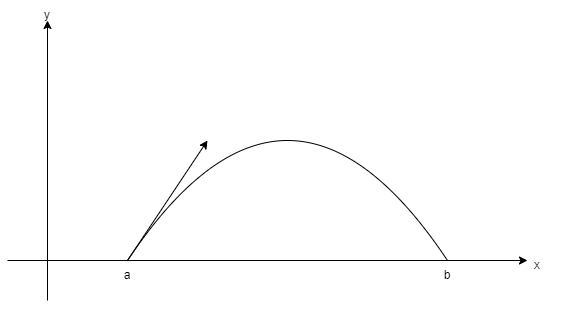
\includegraphics[scale=0.8]{parabola.png}
    \end{figure}

    若將y軸視為高度,將x軸視為水平距離,我們獲得從$x=a$開始到$x=b$的拋物運動軌跡,方向如圖中箭頭所示。回顧速度和距離的關係,可得: \begin{align*}
        x-a=v_x t
    \end{align*}其中$v_x$ 代表水平速度。此算式符合當 $t=0$時, $x=a$的條件,其中 $v_x$ 為常數。設 $t$ 代表時間,則可見垂直與水平運動均取同樣的參數$t$作爲時間參數。如此 \begin{align*}
        v_y=u_y-gt
    \end{align*}
    為能夠適當描述垂直運動的算式,$g$為重力加速度以在算式中表示減速。根據物理學的發現,有如下關係 \begin{align*}
        y=\frac{u_y+v_y}{2}t
    \end{align*} 從而得出 \begin{align*}
        y=u_y t-\frac{1}{2}gt^2
    \end{align*} 再代 $t=\frac{x-a}{v_x}$ 進上述 $y$ 的方程可得如下形式的$x-y$關係以表示抛物綫:\begin{align*}
        y=ax^2+bx+c
    \end{align*}

    爲瞭解抛物綫的性質,引用 \textbf{配方法}:\begin{align*}
        ax^2+bx+c&=a(x^2+\frac{b}{a}x)+c\\
        &=a(x^2+2\frac{b}{2a}x+\frac{b^2}{4a^2}-\frac{b^2}{4a^2})+c\\
        &=a(x+\frac{b}{2a})^2-\frac{b^2-4ac}{4a}\\
        &=a(x+\frac{b}{2a})^2+\frac{4ac-b^2}{4a}
    \end{align*}

    從上述可見當$x+\dfrac{b}{2a}0$時,多項式會到達極值 (極大值或極小值)因爲$(x+\frac{b}{2a})^2$ 的最小值爲 0,同時多項式受 $x+\frac{b}{2a}$所影響擁有頂點。 配方法所得出的形式稱爲 \textbf{頂點式}。從頂點式可總結: \begin{itemize}
        \item \textbf{頂點} 位於 $(-\dfrac{b}{2a},\dfrac{4ac-b^2}{4a})$.
        \item \textbf{對稱軸} 在 $x=-\dfrac{b}{2a}$.
        \item \textbf{極值} 為 $\dfrac{4ac-b^2}{4a}$.
    \end{itemize}

    同時應留意,當圖像擁有極小值時,即有最低點,圖像的開口方向向上:

    \begin{figure}[H]
        \centering
        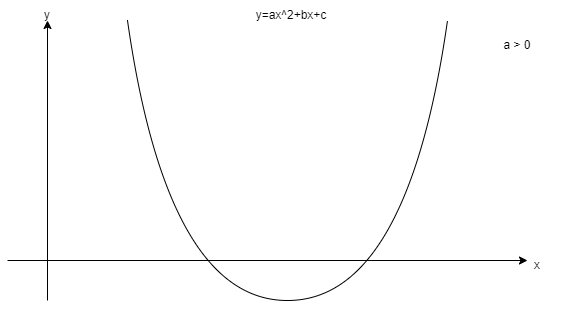
\includegraphics[scale=0.6]{open_upward.png}
    \end{figure}

    而有極大值時,則開口向下:

    \begin{figure}[H]
        \centering
        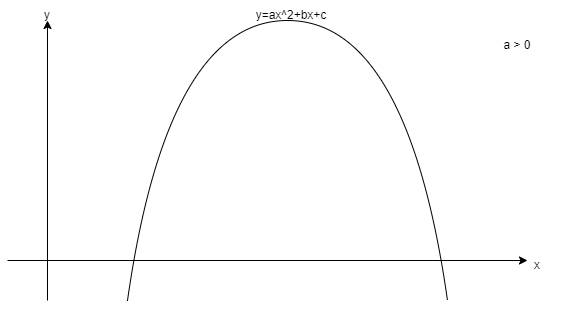
\includegraphics[scale=0.6]{open_downward.png}
    \end{figure}

    \begin{example}
        使用配方法,求$y=2x^2+3x+4$的圖像的開口方向,及頂點坐標、對稱軸和最小值。
    \end{example}

    \textit{ 解.}\begin{align*}
        2x^2+3x+4&=2(x^2+\frac{3}{2}x)+4\\
        &=2(x^2+2\frac{3}{4}x+\frac{9}{16}-\frac{9}{16})+4\\
        &=2(x+\frac{3}{4})^2+\frac{23}{8}
    \end{align*}
    因此,圖像向上開口。其頂點位於$(-\dfrac{3}{4},\dfrac{23}{8})$,對稱軸為 $x=-\dfrac{3}{4}$及最小值為 $\dfrac{23}{8}$。

    \begin{example}
        以$k$ 表$y=kx^2+4x+6$ 的圖像的頂點、對稱軸及極值。
    \end{example}

    \textit{ 解.}
    根據以推導的公式,定點位於 $(-\dfrac{2}{k},\dfrac{4k-4}{k})$,對稱軸位於 $x=-\dfrac{2}{k}$及極值為 $\dfrac{4k-4}{k}$。

    \subsection*{習題}
    \begin{enumerate}
        \item 使用配方法,求以下圖像的開口方向,及頂點坐標、對稱軸和最小值。\begin{align*}
            &a)\ y=2x^2+12x+16&&b)\ y=3x^2+27x+54&&c)\ y=5x^2+35x+30\\
            &d)\ y=7x^2-42x+56&&e)\ y=-11x^2+99x-198&&f)\ y=-3x^2+21x-18
        \end{align*}
        \item 以$k$ 表以下圖像的頂點、對稱軸及極值。\begin{align*}
            &a)\ y=kx^2-2x+9&&b)\ y=82x^2+kx+79&&c)\ y=-24x^2-70x+4k\\
            &d)\ y=-kx^2+36x-k&&e)\ y=8kx^2+3kx-51&&f)\ y=2kx^2+(3k-6)x-4k-8
        \end{align*}
    \end{enumerate}

    \pagebreak

    \subsection*{挑戰題}
    \begin{enumerate}
        \item 解方程 $8x^2+2x+3=2x^2-4$。如有需要,以複數表示答案。
        \item 解方程 $\dfrac{x-3}{2x-3}=\dfrac{7x+3}{2x-5}$。如有需要,以複數表示答案。
        \item 若$x^2-2ax+a^2=0$,求$\dfrac{x}{a}$的值.
        \item $\dfrac{x^{2002}+4x^{2001}}{4x^{2000}}=2449.25$.
        \item 求$\sqrt{6+\sqrt{6+\sqrt{6+\sqrt{6+\cdots}}}}$的准確值。
        \item 若$\alpha,\beta$ 為方程 $x^2-8x+11=0$的根,求 $\alpha^3+\alpha^2+\alpha+\beta^3+\beta^2+\beta$的值。
        \item 若$\alpha,\beta$為以$x$作代數的方程的根: $x^2-5x+a^2-2a+1=0$, 求 $a$ 的值使得$\alpha\beta$達到其最小值。
        \item 求$\alpha^2+\beta^2+\gamma^2$的值,其中 $\alpha,\beta,\gamma$為方程 $3x^3-2x^2+5x-7=0$的根。
        \item 求正實數 $a$的可能值使得$$y=(a^2+1)x^2-2ax+10$$的圖像有極小值$\dfrac{451}{50}$,已知$0<x<\dfrac{1}{2}$。
    \end{enumerate}
\end{document}